\documentclass[xcolor={dvipsnames,table},16pt]{beamer}

\usepackage{lmodern}

\mode<presentation>
{
  \usetheme{UIUC}
}

\usepackage[english]{babel}
\usepackage[utf8]{inputenc}

\usepackage{csquotes}
\usepackage[backend=biber, style=authoryear-comp]{biblatex}
\bibliography{ref.bib}

\RequirePackage{xspace}
\RequirePackage{todonotes}
\RequirePackage[dvipsnames,table]{xcolor}
\usepackage{cancel}

\RequirePackage{listings}
\lstset{
    language=[Sharp]C,
    basicstyle=\small\ttfamily,
    keywordstyle=\color{blue},
    stringstyle=\color{red},
    commentstyle=\color{OliveGreen},
    morekeywords={function},
    numbers=left,
    numberstyle=\small,
    stepnumber=1,
    numbersep=4pt,
    columns=fullflexible,
    breaklines=true,
    breakatwhitespace=false,
    breakindent=1em,
    captionpos=b,
    tabsize=2,
    mathescape=true
}

\RequirePackage{tikz}
\usetikzlibrary{overlay-beamer-styles,backgrounds}
\RequirePackage{multicol}
%\RequirePackage{multirow}

\newcommand{\todoline}[1]{\todo[inline]{#1}}
\newcommand{\myopinion}{\color{Blue}}

\newcommand{\MultiSE}{MultiSE\xspace}
\newcommand{\SymExe}{Symbolic Execution\xspace}
\newcommand{\PathCond}{Path Condition\xsapce}
\newcommand{\ValSum}{Value Summary\xspace}
\newcommand{\ValSums}{Value Summaries\xspace}
\newcommand{\GuardExp}{Guarded Expression\xspace}
\newcommand{\GuardExps}{Guarded Expressions\xspace}
\newcommand{\DynSymExe}{Dynamic \SymExe\xspace}

\newcommand{\TT}{\ensuremath{\mathbf{\mathtt{True}}}\xspace}
\newcommand{\FF}{\ensuremath{\mathbf{\mathtt{False}}}\xspace}

\newcommand{\pc}{\ensuremath{\phi}\xspace} % path constraint


\title[\MultiSE]{\MultiSE: Multi-path Symbolic Execution using Value Summaries}
\author[C. Hsieh]{
   Koushik Sen, George Necula, Liang Gong, Wontae Choi\texorpdfstring{\\}{}
   EECS, UC Berkeley\texorpdfstring{\\}{}
   \texorpdfstring{\bigskip}{\space}
   Presenter: Chiao Hsieh
}
\institute[@ UIUC CS]{}
\date{\today}

\begin{document}

{\nologo
\begin{frame}
\titlepage
\end{frame}
}

\begin{frame}{Motivation}
    \begin{itemize}
        \item \emph{Symbolic Execution} is a key program analysis technique in a variety of applications
        such as Automated Test-case Generation and Program Verification
        \item \emph{Path/State Explosion} problem is one major factor that limits Symbolic Execution to be scalable
        
        \item This paper addresses Path/State Explosion with \emph{\ValSums}
    \end{itemize}
\end{frame}

% Uncomment these lines for an automatically generated outline.
\begin{frame}{Outline}
  \tableofcontents
\end{frame}

\section{Symbolic Execution}\label{sec:sym-exe}

\begin{frame}{\SymExe}

\textit{
``\dots an alternative \underline{``Symbolic Execution'' semantics} for a
programming language where the real data store need not to be used but can be
represented by \underline{arbitrary symbols}.''
}

\medskip

\textit{
``Computational definition for the basic operators of the language are extended
to accept \underline{symbolic inputs} and produce \underline{symbolic formulas as output}.''
} - \cite{King76}

\begin{center}
	\myopinion
    Extended program semantics with program states represented by symbolic inputs
\end{center}

\end{frame}

\begin{frame}[fragile]{(Traditional) \SymExe}

\begin{columns}
\begin{column}{.45\textwidth}

\begin{overlayarea}{\columnwidth}{.8\textheight}

\lstinputlisting{example.cs}

\only<1-6>{
	Concrete execution with $x=30, r=2, z=5$
}\only<7->{

	\only<7>{
	Symbolic execution with symbolic value $x_0, r_0, z_0$
	}\only<8>{
	Symbolic stores:
	
	Symbolic expressions as values
	}\only<9>{
	Assignments:
	
	Update with new semantic of operators to construct symbolic expressions
	}\only<10>{
	Conditional:

	Track path conditions \pc
	
	\alert{Fork} when both branches are feasible,
	concurrently execute both
	}\only<11>{
	Visualized as Symbolic Execution Tree
	
	Program Configuration is the set of Symbolic Stores on frontier nodes 
	}\only<12>{
	(Ideal) path condition \pc:
	
	Assignment $\alpha$ satisfies \pc
	$\iff$ program with input $\alpha$ executes along the path
	}\only<13>{
	Symbolic execution terminates when all forked processes terminate
	}
}

\end{overlayarea}

\end{column}
\begin{column}{.55\textwidth}
\centering
\begin{tikzpicture}[
    overlay, -stealth,
    every node/.style={
    	circle,draw,inner sep=1pt, text centered, minimum height=1em,
    	color=Black
    },
	cond/.style={draw=none, font=\scriptsize},
    desc/.style={draw=none, align=center, font=\tiny,inner sep=0pt},
    node distance=0pt,
	level distance=25pt,
	level 3/.style={sibling distance=30mm},
	level 4/.style={sibling distance=15mm},
	level 5/.style={sibling distance=7mm}
]

\node (1) at (-1, 3) {1}
	child[visible on=<{2-6,8-}>] {node (2) {2}
		child[visible on=<{3-6,9-}>]{node (3) {3}
			child[visible on=<{10-}>]{node (4) {4}
				child[visible on=<{13-}>]{node {5}
					child{node {6}
						child{node {7}
							child{node {8}}
						}
						child{node {\color{red}X}}
					}
				}
				child[visible on=<{13-}>]{node {6}
					child{node {7}
						child{node {8}}
					}
					child{node {8}}
				}
				edge from parent node[cond, left] {$(x > 100)$}
			}
			child[visible on=<{4-6,10-}>]{node (6) {6}
				child[visible on=<{5-6,11-}>]{node (7) {7}
					child[visible on=<{6,12-}>]{node (8) {8}}
	                edge from parent node[cond, left] {$(r > 1)$}
				}
				child[visible on=<{11-}>]{
					node (80) {8}
					edge from parent node[cond, right] {$\neg(r > 1)$}
				}
				edge from parent node[cond, right] {$\neg(x > 100)$}
			}
		}
	}
;

\foreach \Cont in {1,2,3,6,7,8}
    \node[desc, visible on=<+>, left=of \Cont]
    {\footnotesize
    	$\left\{
        \begin{alignedat}{4}
        loc& \mapsto \Cont &,
          r& \mapsto \only<1>{\bot}\only<2->{\alert<2>{2}},\\
          x& \mapsto \only<1>{\bot}\only<2>{\alert<2>{30}}\only<3->{\alert<3>{60}} &,
          z& \mapsto \only<1>{\bot}\only<2-5>{\alert<2>{5}}\only<6>{\alert{1}}
        \end{alignedat}
        \right\}$
    };

    %% SymExe states
   	\arraycolsep=1pt
    
\foreach \Cont in {1,2,3}
    \node[desc, visible on=<+>, right=of \Cont]
    {\footnotesize
    	$\left\{
        \begin{array}{rlrl}
        \multicolumn{4}{c}{\pc \mapsto \TT,}\\
        loc&\mapsto \Cont &,
          r&\mapsto \only<7>{\bot}\only<8-9>{\alert<8>{r_0}},\\
          x&\mapsto \only<7>{\bot}\only<8>{\alert{x_0}}\only<9>{\alert{2x_0}} &,
          z&\mapsto \only<7>{\bot}\only<8-9>{\alert<8>{z_0}}
        \end{array}
        \right\}$
    };

    \node[desc, visible on=<10-12>, below=-1cm of 4]
    {
 	  	$\left\{
		\begin{array}{rlrl}
		\multicolumn{4}{c}{\pc \mapsto \alert{2x_0 > 100},}\\
		loc&\mapsto 6 &,
		r&\mapsto r_0,\\
		x&\mapsto 2x_0 &,
		z&\mapsto z_0
		\end{array}
		\right\}$
    };
	\node[desc, visible on=<10>, below=-1cm of 6]
	{
		$\left\{
		\begin{array}{rlrl}
		\multicolumn{4}{c}{\pc \mapsto \alert{\neg(2x_0 > 100)},}\\
		loc&\mapsto 4 &,
		r&\mapsto r_0,\\
		x&\mapsto 2x_0 &,
		z&\mapsto z_0
		\end{array}
		\right\}$
	};
	\node[desc, visible on=<11>, below left=-5mm of 7]
	{
		$\left\{
		\begin{array}{rlrl}
		\pc & \multicolumn{3}{c}{\mapsto \neg(2x_0 > 100)}\\
		    & \multicolumn{3}{c}{\alert{\land (r_0 > 1)},}\\
		loc&\mapsto 4 &,
		r&\mapsto r_0,\\
		x&\mapsto 2x_0 &,
		z&\mapsto z_0
		\end{array}
		\right\}$
	};
	\node[desc, visible on=<11->, below right=-5mm of 80]
	{
		$\left\{
		\begin{array}{rlrl}
		\pc & \multicolumn{3}{c}{\mapsto \neg(2x_0 > 100)}\\
		& \multicolumn{3}{c}{\alert{\land \neg(r_0 > 1)},}\\
		loc&\mapsto 4 &,
		r&\mapsto r_0,\\
		x&\mapsto 2x_0 &,
		z&\mapsto z_0
		\end{array}
		\right\}$
	};
	\node[desc, visible on=<12->, below=-1cm of 8]
	{
		$\left\{
		\begin{array}{rlrl}
		\pc & \multicolumn{3}{c}{\mapsto \neg(2x_0 > 100)}\\
		& \multicolumn{3}{c}{\alert<12>{\land (r_0 > 1)},}\\
		loc&\mapsto 4 &,
		r&\mapsto r_0,\\
		x&\mapsto 2x_0 &,
		z&\mapsto \alert{r_0-1}
		\end{array}
		\right\}$
	};
\end{tikzpicture}

\end{column}
\end{columns}
\end{frame}

\begin{frame}{Path/State Explosion Problem}

\begin{columns}

\begin{column}{0.55\textwidth}
\begin{overlayarea}{\columnwidth}{.8\textheight}
\footnotesize

$
\begin{array}{l|l|llll}
	     & \pc   & loc & r                                 & x                                     & z       \\ \hline
	M8_1 & \pc_1 & 8   & r_0^2 + 2                         & \only<2>{\cellcolor{Lavender}}2x_0 & r_0^2 + 1  \\
	M8_2 & \pc_2 & 8   & \only<2>{\cellcolor{Lavender}}r_0 & \only<2>{\cellcolor{Lavender}}2x_0 & \only<2>{\cellcolor{YellowGreen}}r_0 - 1 \\
	M8_3 & \pc_3 & 8   & \only<2>{\cellcolor{Lavender}}r_0 & \only<2>{\cellcolor{Lavender}}2x_0 & z_0     \\
	M8_4 & \pc_4 & 8   & \only<2>{\cellcolor{Lavender}}r_0 & \only<2>{\cellcolor{Lavender}}2x_0 & \only<2>{\cellcolor{YellowGreen}}r_0 - 1 \\
	M8_5 & \pc_5 & 8   & \only<2>{\cellcolor{Lavender}}r_0 & \only<2>{\cellcolor{Lavender}}2x_0 & z_0
\end{array}
$

$
\begin{array}{l}
\pc_1 = 2x_0>0 \land z_0 = 1 \land r_0^2 + 2 > 1             \\
\pc_2 = 2x_0>0 \land \neg(z_0 = 1) \land r_0 > 1       \\
\pc_3 = 2x_0>0 \land \neg(z_0 = 1) \land \neg(r_0 > 1) \\
\pc_4 = \neg(2x_0>0) \land (r_0 > 1)                   \\
\pc_5 = \neg(2x_0>0) \land \neg(r_0 > 1)               \\
\end{array}
$

\bigskip

\only<1>{
\# paths can grow exponentially many w.r.t \# branches
for loop-free program

\medskip

\# paths can be infinite for programs w/ loops
}
\only<2>{
Observation:

Symbolic stores of same $loc$ share same symbolic expressions

Redundant \textcolor{Lavender}{stores} and \textcolor{YellowGreen}{computations} among paths
}

\end{overlayarea}
\end{column}
\begin{column}{0.45\textwidth}
\centering
\begin{tikzpicture}[
overlay, -stealth,
every node/.style={circle,draw,inner sep=1pt, text centered, minimum height=1em},
every label/.style={label position=below, rectangle, draw=none, align=center, left},
desc/.style={rectangle, draw=none, align=center, font=\tiny,inner sep=0pt},
node distance=10pt,
level distance=25pt,
level 3/.style={sibling distance=30mm},
level 4/.style={sibling distance=15mm},
level 5/.style={sibling distance=7mm}
]
\node (1) at (0, 3) {1}
child{node (2) {2}
    child{node (3) {3}
        child{node {4}
            child{node {5}
                child{node {6}
                    child{node {7}
                        child{node [label=left:{$M8_1$}] {8}}
                    }
                    child{node {\color{red}X}}
                }
            }
            child{node {6}
                child{node {7}
                    child{node [label={$M8_2$}] {8}}
                }
                child{node [label={$M8_3$}]{8}}
            }
        }
        child{node {6}
            child{node {7}
                child{node [label={$M8_4$}] {8}}
            }
            child{node [label={$M8_5$}] {8}}
        }
    }
}
;
\end{tikzpicture}
\end{column}

\end{columns}

\end{frame}

\begin{frame} {Intuition on State Merging}
\begin{overlayarea}{\textwidth}{.55\textheight}
	\centering
	\begin{tikzpicture}[
	overlay, -stealth,
	every node/.style={circle,draw,inner sep=1pt, text centered, minimum height=1em},
	every label/.style={label position=below, rectangle, draw=none, align=center, left},
	desc/.style={rectangle, draw=none, align=center, font=\tiny,inner sep=0pt},
	node distance=25pt,
	level distance=25pt,
	level 3/.style={sibling distance=30mm},
	level 4/.style={sibling distance=15mm},
	level 5/.style={sibling distance=7mm}
	]

	\node (1) at (-2.5, 0.5) {1}
	child{node (2) {2}
		child{node (3) {3}
			child{node {4}
				child{node {5}
					child{node [label={\only<1>{$M6_1$}}] {6}
						child[visible on=<2->]{node [label={$M7_1$}] {7}
%							child{node [label=left:{$M8_1$}] {8}}
						}
						child[visible on=<2->]{node {\color{red}X}}
					}
				}
				child{node [label={\only<1>{$M6_2$}}] {6}
					child[visible on=<2->]{node [label={$M7_2$}] {7}
%						child{node [label={$M8_2$}] {8}}
					}
					child[visible on=<2>]{node [label={$M8_3$}]{8}}
				}
			}
			child{node [label={\only<1>{$M6_3$}}] {6}
				child[visible on=<2->]{node [label={$M7_3$}] {7}
%					child{node [label={$M8_4$}] {8}}
				}
				child[visible on=<2->]{node [label={$M8_5$}] {8}}
			}
		}
	}
	;
	
	\node [right=5.5 of 1] {1}
	child{node {2}
		child{node (m3) {3}
			child{node (m4) {4}
				child{node (m5) {5}}
				child[invisible]{}
			}
			child[invisible]{}
		}
	}
	;

	\coordinate [below of=m3] (c1)
		child {node [label=right:{\only<2->{\color{Red}}$\widehat{M6}$}] (m6) {6}
			child[visible on=<2>]{node [label={$\widehat{M7}$}] {7}
%				child{node {8}}				
			}
			child[visible on=<2>]{node [label={$\widehat{M8}$}] {8}}
	}
	;

	\draw
	(m3) edge (m6)
	(m4) edge (m6)
	(m5) edge (m6)
	;

	\end{tikzpicture}

\end{overlayarea}
\flushright
\begin{overlayarea}{0.9\textwidth}{.16\textheight}
\only<1>{
	A new representation to approximate some or all frontier symbolic stores at same $loc$.
	
	I.e. $\widehat{M6} \approxeq \{M6_1, M6_2, M6_3\}$
}\only<2>{
	Symbolic Execution with the new representation should preserve the approximation.
	
	I.e. $\widehat{M7} \approxeq \{M7_1, M7_2, M7_3\}$ and
		 $\widehat{M8} \approxeq \{M8_3, M8_5\}$ 
}

\end{overlayarea}
	
\end{frame}

\begin{frame}{Conventional State Merging}

{\footnotesize
$
\begin{array}{l|l|cccc}
	             & \pc                                         & loc & r     & x    & z   \\ \hline
	\only<1>{M6_1}\only<2>{M7_1} & \pc_1 \only<2->{\alert{\land r_0^2+2>1}} & 6   & r_0^2+2   & 2x_0 & z_0 \\
	\only<1>{M6_2}\only<2>{M7_2} & \pc_2 \only<2->{\alert{\land r_0>1}} & 6   & r_0   & 2x_0 & z_0 \\
	\only<1>{M6_3}\only<2>{M7_3} & \pc_3 \only<2->{\alert{\land r_0>1}} & 6   & r_0   & 2x_0 & z_0 \\ \hline \hline
	\widehat{M6} & \widehat{\pc} \equiv 
		\left(\begin{array}{l}
			(\pc_1 \land \textcolor{red}{r_1 = r_0^2 + 2})     \\
			\lor(\pc_2 \land \textcolor{red}{r_1 = r_0}) \\
			\lor(\pc_3 \land \textcolor{red}{r_1 = r_0})
		\end{array}\right)                                     & 6   & \alert{r_1} & 2x_0 & z_0 \\\hline
	\uncover<2->{\widehat{M7} & \widehat{\pc} \land \alert{(r_1 > 1)}     & 7   & \alert{r_1} & 2x_0 & z_0} \\
	\uncover<2->{\widehat{M8} & \widehat{\pc} \land \alert{\neg(r_1 > 1)} & 8   & \alert{r_1} & 2x_0 & z_0}
\end{array}
$}

\begin{overlayarea}{\textwidth}{.29\textheight}
\begin{itemize}
\only<1>{
	\item Add aux variables to path conditions when symbolic expressions are different
    \item Disjunction of path conditions from different paths
    \item Same symbolic execution semantic after merging
}\only<2>{
	\item May introduce predicates with higher complexity to solve
	\begin{itemize}
		\item E.g. $r_0^2+2>1$ in $M7_1$ can be simplified to \TT\\
			  However, we cannot simplify $\widehat{M7}$
	\end{itemize}
	\item Some approaches need to compute joint $loc$ statically
{\myopinion
	and restrict search strategy on symbolic execution tree	
}	% \todoline{cite DSM MergePoint}

}
\end{itemize}
\end{overlayarea}

\end{frame}

\section{MultiSE Algorithm}\label{sec:algo}

\begin{frame}
	\vfill
	\centering
	\usebeamerfont{title}\insertsectionhead
	\vfill
\end{frame}

\begin{frame}[fragile]{\ValSums}
\begin{overlayarea}{\textwidth}{0.39\textheight}
\begin{center}
\footnotesize
$
\begin{array}{@{}l|@{}c@{}c@{}c@{}c@{}}
	              &  loc          & r      & x    & z  \\ \hline
	\Sigma_6 &
		\begin{array}{@{}l@{}}
			\{(\pc_{loc}, 6)\} \text{ where } \\
			\pc_{loc} \equiv \pc_1 \lor \pc_2 \lor \pc_3\\
 		\end{array}
		&
		\left\{
		\begin{array}{@{}l@{}}
			(\pc_1, r_0^2 + 2),\\
			(\pc_2 \lor \pc_3, r_0)
		\end{array} \right\}& \{(\pc_{loc}, 2x_0)\} & \{(\pc_{loc}, z_0)\} \\ \hline

	\Sigma_{78}&
\only<1-2>{
		\left\{
		\begin{array}{@{}l@{}}
			(\pc_{loc} \land \alert{\pc_1 \only<1>{\land \bcancel{(r_0^2 + 2 > 1)}\TT}}, 7), \\
			(\pc_{loc} \land \alert{(\pc_2 \lor \pc_3) \land (r_0 > 1)}, 7), \\
			(\only<2>{\bcancel}{\pc_{loc} \land \alert{\pc_1 \land \only<1>{\bcancel{\neg(r_0^2 + 2 > 1)}}\FF}, 8}), \\
			(\pc_{loc} \land \alert{(\pc_2 \lor \pc_3) \land \neg(r_0 > 1)}, 8)\\
		\end{array}\right\}
}\only<3->{
		\left\{
		\begin{array}{@{}l@{}}
		(
			\left.
			\begin{array}{@{}l@{}}
			\pc_{loc} \land \pc_1 \ \lor \\
			\pc_{loc} \land (\pc_2 \lor \pc_3) \land (r_0 > 1) \\
			\end{array}\right., 7), \\
			\\
		(\pc_{loc} \land (\pc_2 \lor \pc_3) \land \neg(r_0 > 1), 8) \\
		\end{array}\right\}
}
		&
		\left\{
		\begin{array}{@{}l@{}}
		(\pc_1, r_0^2 + 2),\\
		(\pc_2 \lor \pc_3, r_0)
		\end{array}\right\} & \{(\pc_{loc}, 2x_0)\} & \{(\pc_{loc}, z_0)\} \\
\end{array}
$
\end{center}
\end{overlayarea}

\begin{overlayarea}{\textwidth}{.44\textheight}

\only<1>{
    Program configuration $\Sigma$ maps a variable to a \alert{\emph{\ValSum}}\\
    \begin{itemize}    
    	\item A \ValSum is a set of \emph{\GuardExps}\\
	    \item A \GuardExp is a pair of guard \pc and symbolic expression $e$
    	\item Each $(\pc, e) \in \Sigma(r)$ can be regarded as $\pc \land (r_1 = e)$ in last slide
    \end{itemize}
}\only<2>{
    \begin{itemize}
    	\item Merged path condition is encoded by $\pc_{loc}$ in $\Sigma(loc)$
    	\item Operators are extended to accept \textbf{combinations} of \GuardExps
    	\begin{itemize}
    		\item Theoretically \ValSums grow exponentially
    	\end{itemize}
    \end{itemize}
}\only<3->{
	Eager simplification on the value summary of each variable
	\begin{itemize}
		\item Remove $(\pc, v)$ when $\pc \equiv \FF$ (Check UNSATisfiable)
		\item Merge $(\pc, v)$ and $(\pc', v)$ to $(\pc \lor \pc', v)$
		\begin{itemize}
			\item Dynamically merge at joint point (same $loc$ value)
		\end{itemize}
		\item Represent and manipulate guards using Binary Decision Diagram~(BDD)
	\end{itemize}
}
\end{overlayarea}

\end{frame}

\begin{frame}[fragile]{Comparison}

{\footnotesize
$$
\begin{array}{l|c|cccc}
	             & \pc                                         & loc & r     & x    & z   \\ \hline
	\widehat{M6} & \widehat{\pc} \equiv 
	\left(\begin{array}{l}
		(\pc_1 \land \textcolor{red}{r_1 = r_0^2 + 2})     \\
		\lor(\pc_2 \land \textcolor{red}{r_1 = r_0}) \\
		\lor(\pc_3 \land \textcolor{red}{r_1 = r_0})
	\end{array}\right)                                         & 6   & \alert{r_1} & 2x_0 & z_0 \\\hline

	\widehat{M7} & \widehat{\pc} \land \alert{(r_1 > 1)}     & 7   & \alert{r_1} & 2x_0 & z_0 \\
	\widehat{M8} & \widehat{\pc} \land \alert{\neg(r_1 > 1)} & 8   & \alert{r_1} & 2x_0 & z_0
\end{array}
$$

$
\begin{array}{@{}l|@{}c@{}c@{}c@{}c@{}}
			&  loc          & r      & x    & z  \\ \hline
   \Sigma_6 &
		\begin{array}{@{}l@{}}
			\{(\pc_{loc}, 6)\} \text{ where } \\
			\pc_{loc} \equiv \pc_1 \lor \pc_2 \lor \pc_3\\
		\end{array}
		&
		\left\{
		\begin{array}{@{}l@{}}
			(\pc_1, r_0^2 + 2),\\
			(\pc_2 \lor \pc_3, r_0)
		\end{array} \right\}& \{(\pc_{loc}, 2x_0)\} & \{(\pc_{loc}, z_0)\} \\ \hline

\Sigma_{78} &
	\left\{
	\begin{array}{@{}l@{}}
		(\left.
		\begin{array}{@{}l@{}}
			\pc_{loc} \land \pc_1 \ \lor \\
			\pc_{loc} \land (\pc_2 \lor \pc_3) \land (r_0 > 1) \\
		\end{array}\right., 7), \\
		(\pc_{loc} \land(\pc_2 \lor \pc_3) \land \neg(r_0 > 1), 8), \\
	\end{array}
	\right\}
	&
	\left\{
	\begin{array}{@{}l@{}}
		(\pc_1, r_0^2 + 2),\\
		(\pc_2 \lor \pc_3, r_0)
	\end{array}\right\} & \{(\pc_{loc}, 2x_0)\} & \{(\pc_{loc}, z_0)\} \\
\end{array}
$}

Benefits of Value Summaries
\begin{itemize}
	\item Avoid predicate $r_1 = r_0^2 + 2$
	\myopinion
	\item Explicitly exclude infeasible path $r_1 = r_0^2 + 2 \land \neg (r_1 > 1)$
	\item Can possibly simplify $\pc_{loc}$ to \TT
\end{itemize}

\end{frame}

\begin{frame}{BDD Representation for Guards}
	
	\begin{itemize}
		
		\item Represent Boolean formulas using Binary Decision Diagram~(BDD)
		
		\begin{itemize}
			\item Check UNSAT with BDD before UNSAT with SMT solver
			{\myopinion
				\item Mapping from predicates to Boolean variables\\
				E.g. $\pc = \neg(2x_0 > 0) \land (r_0 > 1)$ \\
				Let $(2x_0 > 0) \mapsto b_1$ and $(r_0 > 1) \mapsto b_2$ \\
				BDD stores the formula $\neg b_1 \land b_2$
				\item This is a SAT-preserving transformation to Boolean formula
			}
		\end{itemize}

		\item Benefits of using BDD

		\begin{itemize}
			\myopinion
			\item Simplify and canonicalize Boolean formula by construction
			\item Fast UNSAT checking
			\begin{itemize}
				\myopinion
				\item Detect infeasible paths with UNSAT path conditions
				\item Remove \GuardExps with UNSAT guards
			\end{itemize}
		\end{itemize}
	\end{itemize}
\end{frame}

\section{Implementation}\label{sec:impl}

\begin{frame}{Implementation}
	\MultiSE execution for JavaScript using the Jalangi framework
	\begin{itemize}
		\item \url{https://github.com/SRA-SiliconValley/jalangi/tree/multise}
		\item SMT Solver: CVC3
		\begin{itemize}
			\item Theory of Linear Integer Arithmetic and Strings
		\end{itemize}
		\item BDD Package: author implemented
	\end{itemize}
\end{frame}

\section{Evaluation}\label{sec:eval}

\begin{frame}{Evaluation Setup}

Experiment Environment
\begin{itemize}
	\item Laptop with 2.3 GHz Intel Core i7 and 16 GB RAM
\end{itemize}

Benchmark
\begin{itemize}
	\item 15 JavaScript programs provided by authors
\end{itemize}

Research Questions
\begin{itemize}
	\item RQ1: Effectiveness of sharing using \ValSums
	\item RQ2: Runtime cost of \MultiSE among its components 
	\item RQ3: Performance gains compared to traditional SE
	\item RQ4: Increase on \emph{precise} state merging compared to CSM
	\begin{itemize}
		\item Imprecise state merging happens when unsupported predicates appear in path conditions
	\end{itemize}
\end{itemize}

\end{frame}

\begin{frame}{Evaluation}
    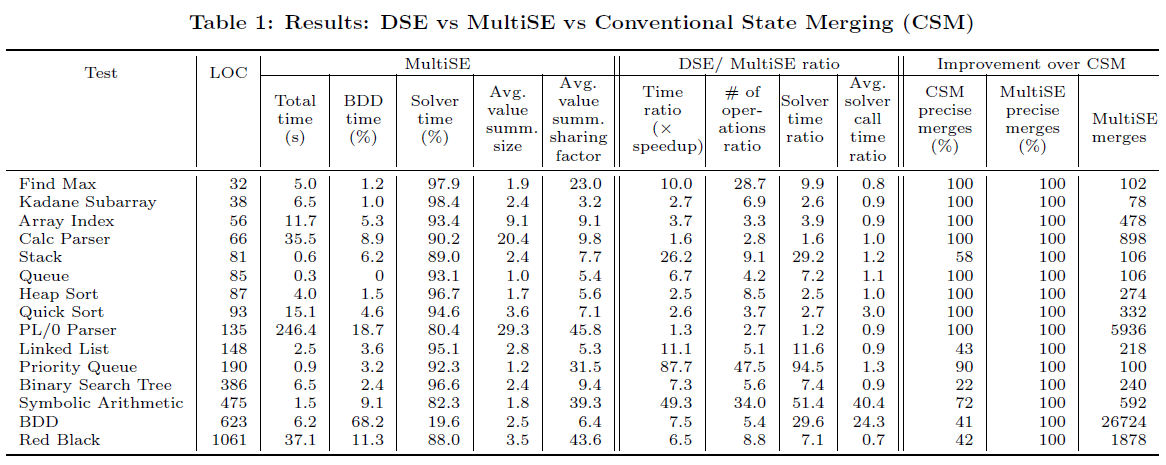
\includegraphics[width=\textwidth]{evaluation.png}
	\begin{itemize}
	\only<1>{
		\item RQ1: Average Size of \ValSum for each variable is between 1-30 
			  and \# Paths/Size ratio shows that the sharing is effective
		\item RQ2: BDD query is actually negligible in most benchmarks
	}\only<2>{
		\item RQ3: Speed up due to much less solver queries using \ValSum
		\item RQ4: Large amount of imprecise merges in CSM in some benchmarks
	} 
	\end{itemize}
\end{frame}

\section{Conclusion}

\begin{frame}{Conclusion}
	\begin{itemize}
		\item \ValSums maintain symbolic values separated from path conditions
		\begin{itemize}
			\myopinion
			\item Symbolic values not used in if-condition does not complicate
			      path conditions
			\item If symbolic values is used in if-condition,
			      the path condition may still be simplified for infeasible paths
		\end{itemize}
		\item \MultiSE dynamically finds and merges at joint points
		\begin{itemize}
			\myopinion
			\item More search strategies are applicable
		\end{itemize}

		\item Evaluation shows size of \ValSums normally is much less than \# Paths
	\end{itemize} 
\end{frame}

\begin{frame}
    \printbibliography
\end{frame}

\appendix

\section*{Appendices}

\begin{frame}{My Questions}
\begin{itemize}
	\item How would different search strategies on SE Tree affects \MultiSE?
\end{itemize}
\end{frame}

%\begin{frame}{\SymExe Variants}
%    \begin{itemize}
%        \item (Static) \SymExe
%        \item \DynSymExe a.k.a. Concolic Testing
%    \end{itemize}
%    \todoline{Cite DART CUTE}
%\end{frame}
%
%\begin{frame}{\SymExe Semantics}
%
%\end{frame}

\begin{frame}{\MultiSE Semantics}

	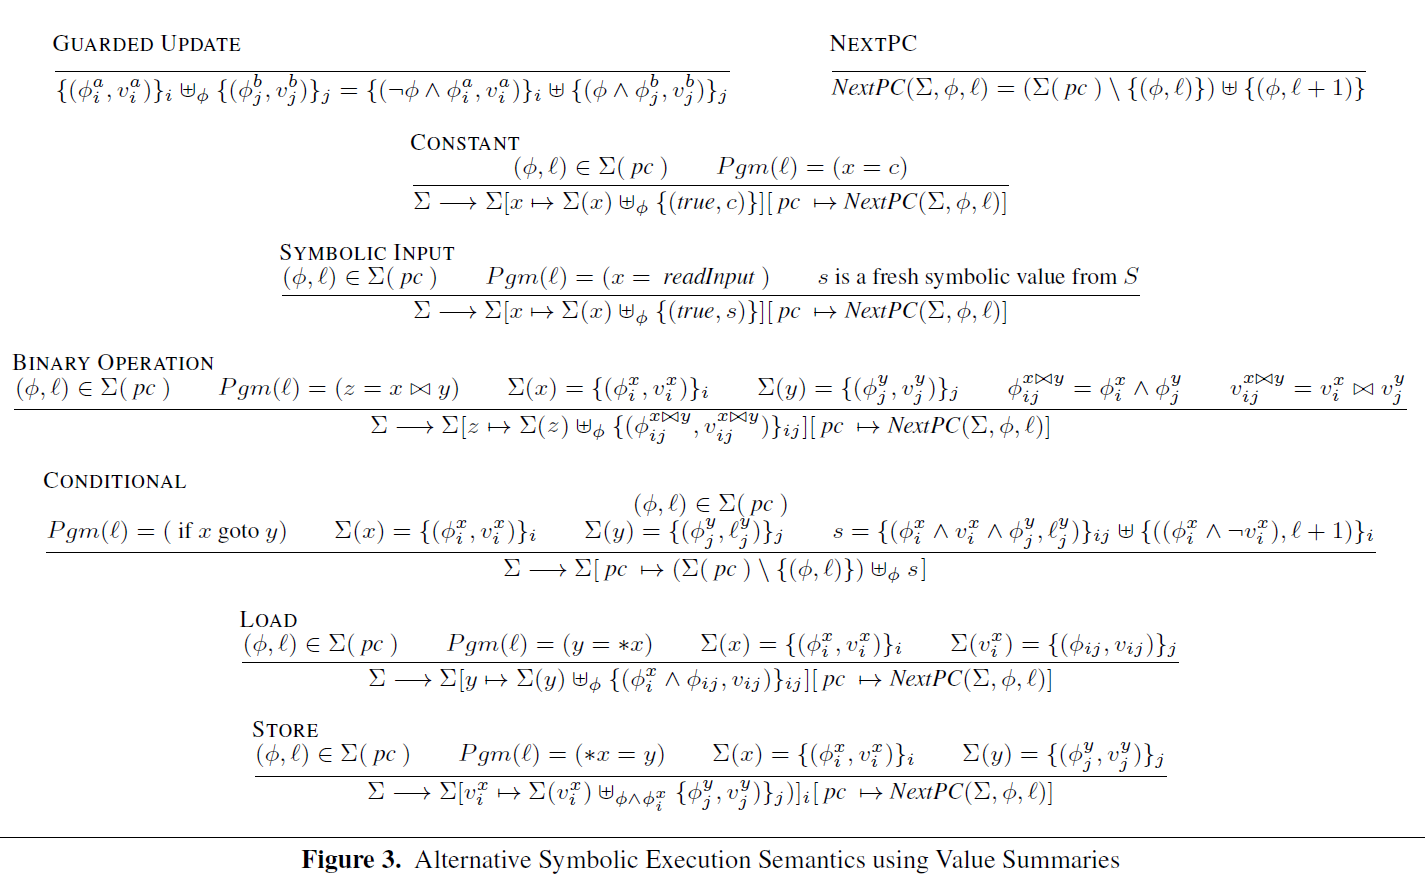
\includegraphics[width=\textwidth]{semantics.png}

\end{frame}

\end{document}
